\documentclass{article} % Tạo một bản báo cáo
\usepackage[document]{ragged2e}
\usepackage{sectsty}
\usepackage[utf8]{inputenc}
\usepackage[T5]{fontenc} % Để sử dụng Tiếng Việt
\usepackage[fontsize=13pt]{scrextend} % Set fontsize=13pt
\usepackage[paperheight=29.7cm,paperwidth=21cm,right=2cm,left=3cm,top=2cm,bottom=2.5cm]{geometry}% Chuẩn A4, căn lề phải, trái, trên, dưới.
%\usepackage[paperheight=29.7cm,paperwidth=21cm,right=2cm,left=3cm,top=2cm,bottom=2.5cm,twoside]{geometry}% Chuẩn A4, căn lề phải, trái, trên, dưới.
\usepackage{mathptmx} % Time New Roman
\usepackage{graphicx} % Thư viện chèn ảnh
\usepackage{float} % Set vị trí chèn ảnh
\usepackage{tikz} % Thư viện tạo khung bìa
\usetikzlibrary{calc} % Thư viện tikz
\usepackage{pifont}
\DeclareUnicodeCharacter{10048}{ \ding{95} } %russian
\DeclareUnicodeCharacter{10051}{ \ding{93} }
%Russian-specific packages
 \usepackage{multirow}
 

\renewcommand{\baselinestretch}{1.2}
\setlength{\parskip}{6pt} % Spacing after
\setlength{\parindent}{1cm} % Set khoảng cách thụt đầu dòng mỗi đoạn
\usepackage{titlesec} % Thư viện để set up các kiểu chữ
\setcounter{secnumdepth}{4} % 4 Heading
\titlespacing*{\section}{0pt}{0pt}{30pt} % Heading 1
\titleformat*{\section}{\fontsize{16pt}{0pt}\selectfont \bfseries \centering}
%raggedright
\titlelabel{\thetitle.\quad}
\titlespacing*{\subsection}{0pt}{6pt}{0pt} % Heading 2
\titleformat*{\subsection}{\fontsize{14pt}{0pt}\selectfont \bfseries}

\titlespacing*{\subsubsection}{0pt}{6pt}{0pt} % Heading 3
\titleformat*{\subsubsection}{\fontsize{13pt}{0pt}\selectfont \bfseries \itshape}

\titlespacing*{\paragraph}{0pt}{0pt}{0pt} % Heading 4
\titleformat*{\paragraph}{\fontsize{13pt}{0pt}\selectfont \itshape}




\begin{document}

\begin{titlepage}
\begin{tikzpicture}[overlay,remember picture]


\draw [line width=3pt]
    ($ (current page.north west) + (3.0cm,-2.0cm) $)
    rectangle
    ($ (current page.south east) + (-2.0cm,2.5cm) $);
\draw [line width=0.5pt]
    ($ (current page.north west) + (3.1cm,-2.1cm) $)
    rectangle
    ($ (current page.south east) + (-2.1cm,2.6cm) $); 
\end{tikzpicture}

\begin{center}
\vspace{-12pt}  Hanoi University of Science and Technology \\
\textbf{\fontsize{16pt}{0pt}\selectfont School of Mechanical Engineering}
\vspace{0.5cm}
 \begin{figure}[H]
     \centering
     
\includegraphics[width=1.53cm,height=2.26cm]{Image/682px-Logo_Đại_học_Bách_Khoa_Hà_Nội.svg.png}
 \end{figure}
\vspace{1.5cm}
\fontsize{24pt}{0pt}\selectfont THESIS\\
\vspace{24pt}
\textbf{\fontsize{32pt}{0pt}\selectfont Mechanical Design Project I}
\vspace{1.5cm}
\end{center}
\hspace{6pt}\textbf{\fontsize{14pt}{0pt}\selectfont Topic:}
\begin{center}
    \textbf{\fontsize{20pt}{0pt}\selectfont DRIVE SYSTEM DESIGN FOR ELEVATORS}\\
    

\vspace{1.5cm}
\begin{table}[H]
    \centering
    \begin{tabular}{l l}
 \fontsize{14pt}{0pt}\selectfont Student:    & \fontsize{14pt}{0pt}\selectfont Ha Luc Minh Vu \\
 \fontsize{14pt}{0pt}\selectfont Student ID:  & \fontsize{14pt}{0pt}\selectfont 20185317
 
 \vspace{6pt} \\ 
     &\fontsize{14pt}{0pt}\selectfont Advanced Program of Mechatronics 01 – K63 \vspace{6pt}\\
\fontsize{14pt}{0pt}\selectfont Instructor:  & \fontsize{14pt}{0pt}\selectfont Prof. Dr. Le Minh Quy \\
\fontsize{14pt}{0pt}\selectfont Course code: &
\fontsize{14pt}{0pt}\selectfont ME3066
\end{tabular}
\end{table}
\vspace{5cm}
 \fontsize{14pt}{0pt}\selectfont Hanoi - 2022
\end{center}
\cleardoublepage


\thispagestyle{empty}

\cleardoublepage
 % Tạo mục lục tự động
\addtocontents{toc}{\protect\thispagestyle{empty}}
\tableofcontents 
\thispagestyle{empty}
\cleardoublepage
\pagenumbering{roman} % Đánh số thứ tự la mã
\section*{LIST OF SYMBOLS AND ABBREVIATIONS}
\phantomsection \addcontentsline{toc}{section}{\numberline {} LIST OF SYMBOLS AND ABBREVIATIONS}

\begin{tabular}{ l l }
\hspace{1cm} AWGN & \hspace{4cm} Additive White Gaussian Noise \\  
\hspace{1cm} BC & \hspace{4cm} Broadcast Channel    \\
\hspace{1cm} BS  & \hspace{4cm} Base Station\\
\hspace{1cm} CSI & \hspace{4cm} Channel State Information \\  
\end{tabular}  

\newpage % Danh mục ký hiệu và chữ viết 


%Tạo danh mục hình vẽ.
{\let\oldnumberline\numberline
\renewcommand{\numberline}{Figure~\oldnumberline}
\listoffigures} 
\phantomsection\addcontentsline{toc}{section}{\numberline {} LIST OF FIGURES}
\newpage

 %Tạo danh mục bảng biểu.
{\let\oldnumberline\numberline
\renewcommand{\numberline}{Bảng~\oldnumberline}
\listoftables}
\phantomsection\addcontentsline{toc}{section}{\numberline {} LIST OF TABLES}
\newpage
\justifying
%\section*{Abstract}

\newpage
\pagenumbering{arabic} % Đánh số thứ tự 1,2,3...
\section*{CHAPTER 1\\ \vspace{0.5cm} PARAMETERS ANALYSIS OF THE ELEVATORS}
\addcontentsline{toc}{section}{\numberline{}CHAPTER 1\\ \vspace{0.5cm} PARAMETERS ANALYSIS OF THE ELEVATORS}



\section{Structure of the elevators}

    

The mechanical structure of an elevator basically consists of a driving motor, a gear box, an elevator car, a counterweight, and cables. The driving motor is used to generate motion for the gear box; meanwhile, gearbox can convert high speed, small torque to the higher torque, appropriate speed for the big main sheave. The counterweight and the car are almost the same in weight; they are hoisted by the cables and the car carries passengers.




I, Structure of elevators

1.  Fixed devices in elevator wells\\
1.1  Guide Rail

Guide rails are installed along the cab and the counterweight moves along the well. And make sure the cabin and counterweight are always in the designed position in the well and the frame is displaced horizontally during movement.\\
1.2  Buffer

Installed under the pit to stop and support the car in case the cabin or counterweight moves downwards beyond the position of the bottom travel limit switch.

2. Cabin and related equipment

The cab is the load-carrying part of the elevator. The cab shall be constructed so that small parts can be assembled and disassembled. According to the structure, the cabin consists of 2 parts: the bearing structure (cabin frame) and the covering lines, ceiling and floor forming the cabin chamber.\\

2.1 Cabin frame

Elevator cabin is the position we stand in the process of use. In particular, the cabin frame has a bearing role for the entire elevator load. This means that this is the main part that determines the efficiency and safety of the device.\\
2.2 Guide shoe\\

It has the effect of guiding the cabin and the counterweight moving along the guide rail and controlling the horizontal displacement of the car and the counterweight in the well to not exceed the allowable value. There are 2 types of guide mounts:
•	Guide shoe 
•	Roller guide shoe\\

2.3 Cabin suspension

Since the cabin and counterweight are suspended by separate cables, the suspension system must be bent to ensure that these separate lifting cables have the same tension, otherwise it will be very dangerous. Therefore, the car suspension system must be equipped with an electrical contact of the safety circuit to cut off the power to stop the ladder when one of the cables is too loose to prevent accidents.

2.4 Cabin

The cabin is a removable structure consisting of the ceiling, floor and wall of the car. These parts are linked to the bearing frame of the cabin.

2.5 System of cabin doors and floors

Cabin doors and landing doors are parts that play a very important role in ensuring safety and greatly affect the quality and productivity of the elevator.

3. Elevator balancing system

Stabilization system in the elevator to balance the car weight and lifting load. The choice of the kinematic scheme and the weight of the components of the balancer system greatly affects the load torque and motor power of the drive mechanism, the maximum tension of the lifting rope and the pulling capacity of the pulley. Friction .Elevator balancing system includes:
3.1  Counterweight

For heavy lift lifts, the counterweight and the cabin are suspended by a cable hoist and then the upper girder of the counterweight frame has the pulleys of the cable hoist system.
3.2  Lifting cable

The cable is grounded from fine carbon fibres, with a tensile strength of 1400-1800 N/mm2. Steel wires fabricated by cold drawing technology have a diameter of 0.5 to 2-3 mm and are braided into cables using specialized braiding equipment.
3.3  Chain and balance cable

When the lift has a lifting height of more than 45 m or the weight of the lifting cable and electric cable is more than 0.1 Q, an additional cable or balance chain must be placed to reduce the weight of the lifting cable and power cable. switch from the cabin suspension branch to the counterweight branch and vice versa when the elevator operates, ensuring a relatively stable load torque on the friction pulley.
4.  Machine drive

Depending on the drive scheme, the elevator's winch unit is located in the driving machine room, located above, below or next to the well.
Depending on the drive method, two types are:
•	Hydraulic puller.
•	Electric puller . 

5.  Mechanical safety device

The mechanical safety device in the elevator has a role to ensure the safety of the elevator and passengers in the event of an incident such as: cable breakage, cable slip on the friction pulley groove, the cabin is lowered at a speed exceeding the rack. allowable value. The mechanical safety device in the elevator consists of 2 main components:
5.1  Safety Gear

Includes 3 types:
•	Instant-acting safety gear connected to the lifting cable.
•	Instant-acting insurance gear with speed limiter.
•	Quiet acting insurance gear.

5.2  Overspeed Governor

When the car is lowered at a speed exceeding the allowable value, the speed limiter through the lever system acts on the safety brake to stop the car resting on the guide rails. The allowable value of the car lowering speed is taken depending on the type of lift as specified in the standard.
II, Working principle 

When the motor rotates to rotate the pulley, the pulley will make the rope move and pull the elevator car to move in the preset direction, when the motor rotates in the opposite direction, the pulley will rotate in the opposite direction and cause The elevator cab moves in the opposite direction to the predetermined direction.
III, Select the motion module of the elevator


1. Elevator classification

Today's elevators are designed and manufactured in a variety of ways, with many models, different types to suit the intended use of each project.
* Elevators can be classified according to the following principles and characteristics:
1.1 According to use (TCVN 5744 ~1993) elevators are classified into 5 types

a.  Elevator carrying people:
This type is specialized for transporting passengers in hotels, motels, apartment buildings, schools, etc.
b.  Passenger lifts with regard to accompanying goods:
This type is often built for supermarkets, exhibition areas, etc.
c.  Dedicated elevator waiting for patients:
This type is built specifically for hospitals, nursing homes.... Its characteristic is that the cabin's size must be large enough to accommodate the patient's stretcher (stretch) or bed, along with the doctors. staff and accompanying first aid equipment. Currently in the world it is manufactured according to the same size and load standards for this type of elevator.
d.  Cargo lifts with chaperones:
This type is often erected in factories, factories, warehouses, ladders used for hotel staff, etc., mainly built to carry goods but accompanied by people to serve.
e.  Unaccompanied cargo elevator:
Specialized type to carry materials. food in hotels, etc. The feature of this type is that only the control stroke is outside the cabin (in front of the landing doors), while other types of ladders can be controlled both inside and outside the cabin if above.
1.2 According to the cabin drive system

a.	Electric drive lifts:

The type of ladder that drives the cabin up and down thanks to the electric motor transmitted through the reducer to the friction pulley or the cable escalator. It is thanks to the cabin that is suspended by a cable that its journey up and down is not restricted. There is also a ladder that drives the cabin up and down thanks to a rack gear.
b. Hydraulic lift (by cylinder - piston):
The feature of this type of ladder is that the cabin is pushed from the bottom by a piston-hydraulic cylinder, so the travel is limited. Currently, hydraulic elevators with a maximum stroke of about 18 m, so it cannot be equipped for high-rise buildings, despite the simple structure, saving the well when having the same load compared to the guide. cable motor, smooth and safe movement, reducing the overall height of the building when having the same service floor, and the engine room on the ground floor.
c. Pneumatic elevator

2.  Select a module

According to the above and below parameters, I choose the elevator's motion module as electric drive.
\newpage




\begin{figure}[!ht]
    \centering
     % \centerline{\includegraphics[width=1.1\textwidth, height = 1.5cm]{s_TTCD_data.png}}
   \centerline{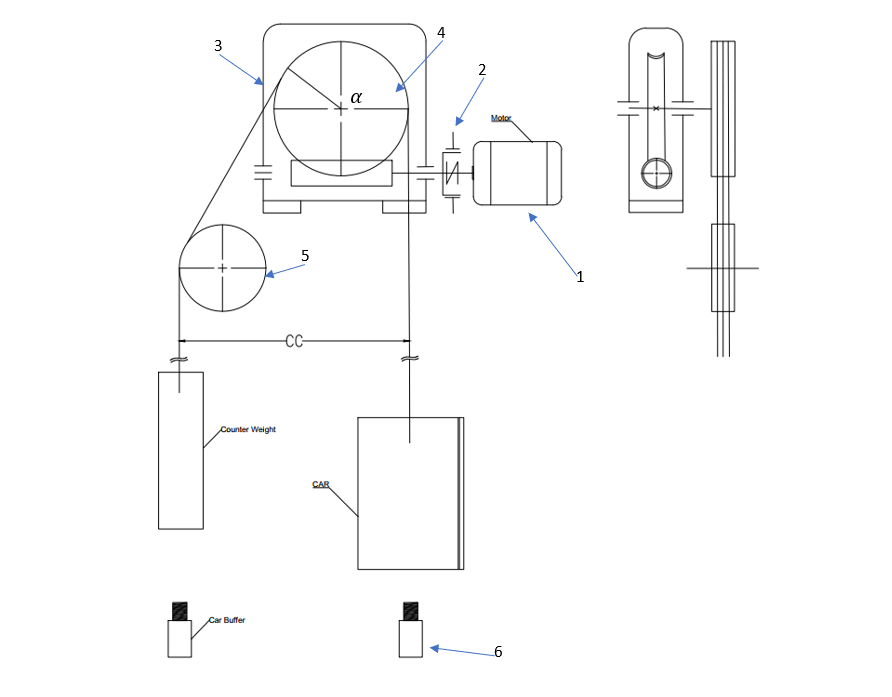
\includegraphics[width=21cm,height=16.8cm]{Image/so do co cau.png}}
    \caption[Dynamic diagram]{\bfseries \fontsize{12pt}{0pt}\selectfont Dynamic diagram}
    \label{figure1}
\end{figure}
\vspace{19.2cm}

\begin{table}[H]
    \centering
    
    \begin{tabular}{l l}
        \fontsize{12pt}{0pt}\selectfont 1.     \fontsize{12pt}{0pt}\selectfont Motor \\
        \fontsize{12pt}{0pt}\selectfont 2.   \fontsize{12pt}{0pt}\selectfont Flexible coupling\\
        \fontsize{12pt}{0pt}\selectfont 3.     \fontsize{12pt}{0pt}\selectfont Gearbox \\
        \fontsize{12pt}{0pt}\selectfont 4.     \fontsize{12pt}{0pt}\selectfont Pulley \\
        \fontsize{12pt}{0pt}\selectfont 5.     \fontsize{12pt}{0pt}\selectfont Orienting pulley \\

\end{tabular}
\end{table}

\section{Working principle of the elevators}

As the motor is activated by the users, its rotation is transmitted to the main sheave by the gear box. By the balanced-hoisting mechanism including the counterweight and the car, the gearbox therefore can easily move the car upward or downward. When the car shifts upward the counterweight is in downward motion and vice versa. The car stops at selected floor for carrying purposes.
To reduce the noise during operating time of the elevator, the gearbox should use the worm gear transmission. Worm gear transmission has the advantage of high gear ratio, small size and self braking.
Worm gear box can use the cylindrical worm or globoidal worm. Globoidal worm gear are widely used for elevator machines thanks to its smaller dimensions in comparison to the cylindrical type with the same power rating. 
The worm gear box can be manufactured with the worm placed above or below the worm gear. Traction sheave is attached directly to the worm. The wear of the traction sheave is usually high; therefore the sheave collar should be easily disassembled for replacement. The shaft of the worm is placed on the bearing. At an end of the worm which is opposite to the motor, a hand crank is attached so that we can control the machine manually. It is also removable.

\newpage 
\newpage
%\pagenumbering{arabic} % Đánh số thứ tự 1,2,3...
\section*{CHAPTER 2\\ \vspace{0.5cm} CALCULATIONS AND DESIGN}
\addcontentsline{toc}{section}{\numberline{}CHAPTER 2\\ \vspace{0.5cm} CALCULATIONS AND DESIGN}


\begin{table}[H]
    
    \begin{tabular}{l l}
        \fontsize{12pt}{0pt}\selectfont 1. Load: & 
        $ Q_1 =400 \emph{ kg} = 4000\emph{ N} $ \\
        \fontsize{12pt}{0pt}\selectfont 2. Weight of cabinet & 
        G  = 300  \emph{kg} = 3000 \emph{N} \\
         \fontsize{12pt}{0pt}\selectfont 3. Car velocity: & 
        $ V = 10 \emph{ m/min} = 0.167 \emph{ m/s} $ (low speed) \\
        \fontsize{12pt}{0pt}\selectfont 4.	Lifespan: & 
        $ L_h = 16000 $ hours = 4000 \\
         \fontsize{12pt}{0pt}\selectfont 5.	Contact angle between pulley and sheave: & 
        $ \alpha = 137 $ degree  \\
        \fontsize{12pt}{0pt}\selectfont 6.	Distance between two branches of cable:  & 
        $ cc = 1000 $ mm  \\
        \fontsize{12pt}{0pt}\selectfont 7.	Operating condition:  &
        smoothly \\
        \fontsize{12pt}{0pt}\selectfont
        $ Q_m = 2Q_1 = 1750\: kg = 17500\:N$\\
        $ Q_2 = 0,6Q_1 = 240\: kg = 2400\: N$\\
        $ t_1  = 1,9 \:  min $\\
        $t_2  = 2,1  min \:  $ \\
        $t_ck = 3×( t_1 + t_2) = 12 \;  min$\\
\end{tabular}
\end{table}
    

%\section{Computation of driving motor }
\section{Computation of driving motor}
\subsection{Required power on friction pulley shaft}
$$ P_{pl}=\frac{F\times v_d}{1000}=\frac{2602.15\times0.167}{1000}=0.435 (kW)$$\\
In which:\\
$$F = \frac{(1-\varphi)Q_1}{a\eta_g}=\frac{\left(1-0,395\right)\times4000}{1\times0,93}=2602,15 (N)$$
With, weight factor :
$$  \varphi = \frac{\gamma}{2}=\frac{0.79}{2}=0,395 $$ 
Fill factor:
$$\gamma=\frac{Q_1\times t_1+Q_2\times t_2}{Q_1(t_1+t_2)}=\frac{4000\times1.9+2400\times2.1}{4000\times(1.9+2.1)}=0,79  $$

\begin{table}[H]
    \centering
    \begin{tabular}{l l}
    a \; =  1 since car is hoisted directly by the cables\\
	$\eta_g= 0,95 - fz_u = 0,95 - 0,02×1 = 0,93 $\\
	f \;= 0,02 because of using bearing	\\
	$z_u = 1$ since a shaft is oriented - changed\\
    $v_d=a.v=0,167 m/s$\\
    \end{tabular}
\end{table}
\subsection{Required power of motor} 
$$Pr = \frac{P_{pl}}{\eta}=\frac{0,435}{0,792}=0,549\ (kW)$$
Efficiency of transmission system:
$$\eta =\eta_k\times\eta_{tv}\times (\eta_{ol})^2$$
The value of above efficiencies are taken from table 2.3 with:
\begin{table}[H]
    \centering
    \begin{tabular}{l l} 
$\eta_k: $ efficiency of coupling, $\eta_{k}$ =1;\\
$\eta_{ol}: $ efficiency of bearing, $\eta_{ol}$ = 0.995\\
$\eta_{tv}: $ efficiency of one pair worm gear transmission\\
    \end{tabular}
\end{table}
Number of thread $z_1$=2 should choose  $\eta_{tv}$ =0.8
$$\Rightarrow\eta = 1 \times0.8 \times 0.995^2 = 0.792$$
\section{Determine the speed of motor}
\subsection{Selection of pulley diameter}
The number of branches of the cables $Z_c$ =3\\
Tension force on the cables:\\
$$S=\frac{Q_1+G}{a\eta_gz_c}=\frac{4000+3000}{1\times\ 0,93\times\ 3}=2508,96 (N)$$
Tension force on the cables following safety factor\\
Required breaking force:
$$S_{d,yc} = \ Z_p.S=12\times\ 2508,96=30108 (N) $$
In table 2.3, with Sđ $ \geq Sd,yc  => d_c = 12 mm $ \\
The diameter of the pulley shaft D $ \geq 40d_c =40\times12 = 480 (mm) $
\subsection{Estimation of pulley shaft speed }
$$n_{pl}=\frac{60000.a.v}{\pi.D}=\frac{60000\times0,167}{\pi.480}=7 (rpm)$$ \\
\subsection{Estimation of transmission ratio}

\subsection{Estimation of motor speed}
$$n_{sb}=n_{pl}.u_{sb}=7\times 40 = 280 (rpm)$$
\section {Selection of motor}
We select the motor which has the nearest value of power. \\
In table P.1.3 [1] with: \\
        	 $$	 P_r = 0.549 (kW) \;\;\; and \;\;\;\;
         		 n_{db} = 750 (rpm) $$
We now can choose motor 4A90LA8Y3 with the following parameters: 
\begin{table}[H]
    \centering
    \begin{tabular}{l l}
        $	P_{dc} = 0.75 (kW) $  \\
        $ n_{dc} = 705 (rpm)   $ \\
        $\frac{T_k}{T_{dn}}= 1,6$ \\
        $m_{dc} = 28.7   (kg)  $\\ 
        $d_{dc} =  24 (mm) $\\
    \end{tabular}
\end{table}

  
\section{Determine speed, power, moment of shafts}
\subsection{	Recalculate transmission ratio }
Actual transmission ratio of the system 
$$u_t=\frac{n_{dc}}{n_{pl}}=\frac{705}{7}=100.7$$
Then $u_t = 100.7$
\subsection{Determine dynamic parameters of gearbox }
Speed of shafts
$n_1=n_{dc}=705 (rpm)$
$$n_2=\frac{n_1}{u_{tv}}=\frac{705}{100.7}=7 (rpm)$$
Power on shafts 
$$p_2= P_{pl}= 0.435 (KW)$$
$$p_1=\frac{p_2}{\eta_{tv}\eta_{ol}}=\frac{0.435}{0,8\times0,995}=0.546 (kW) $$
$$p_{dc}=\frac{p_1}{\eta_k\eta_{ol}}=\frac{0.546}{1\times0,995}=0.549  (kW) $$
	Moment on shafts
$$T_{dc}=9,55.10^6\frac{p_{dc}}{n_{dc}}=9.55\times10^6\frac{0.75}{705}=10159.57  (N.mm) $$
$$ T1=9,55.10^6\times\frac{p_1}{n_1}=9,55\times10^6\frac{0.546}{705}=7396.17 (N.mm) $$
$$ T2=9,55.10^6\times\frac{p_2}{n_2}=9,55\times10^6\frac{0.435}{7}=593464.29  (N.mm) $$      

\begin{table}[h!]
  \begin{center}
   % \caption{More columns.}
    \label{tab:table1}
     \begin{tabular}{l|S|S|l}
      \textbf{Transmission ratio} & \textbf{Motor shaft} & \textbf{Shaft I } & \textbf{Shaft II}\\ % <-- added & and content for each column
      
       & 1 &  & 35.05 \\ % <--
      \hline
      P (kW) & 0.549 & 0.546 & 0.435\\ % <--
      n (rpm) & 705 & 705 & 7\\ % <--
      T (N.mm) & 10159.57   & 7396.17 & 593464.29  \\ % <--
    \end{tabular}
  \end{center}
\end{table}


\section {Computation of transmission system}
\subsection{Input}
	
	Torsion on driven shaft: T2 = 593464.29 (Nmm) = 593.46 (Nm)\\
	Speed of rotation on drive shaft: $n_1 = 705 $(rpm) \\
	Transmission ratio : $u=u_{tv} = 100.7 $ \\
	Required lifespan:$ L_h = 30000 (hours) $
	Relationship between load modes :
$$T_{ck} = 3(t1 + t2) = 3(1.9 + 2.1) = 12 (min)$$
$$\frac{t_2}{t_1}=\frac{2.1}{1.9}=\frac{21}{19}$$
$$\frac{Q_2}{Q_1}=0.6$$
$$\frac{Q_m}{Q_1}=2$$

 Operating condition : quiet  %center

\subsection{Selection of materials and determining allowable stress }
\subsubsection{	Material selection}
Sliding gear:
$$	v_S={4,5.10}^{-5}.n_1.\sqrt[3]{593464.29} = 2.67 (m/s) $$ 
Because $v_S < 5(m/s)$, we use bronze with no tin to make worm gear. Specifically, brass \\
-	Symbol : \;\; $Б$pA \;\; 9-4\\
-	Casting method : using metal molds\\
-	$\sigma_b$ = 340 (MPa)    	\\	
-	$\sigma_{ch}$ = 140 (MPa)    



\subsection{Determination of allowable stresses of worm gear }

\subsubsection{Allowable contact stress }
With $v_s$ = 2.67 m/s and the worm gear is made by brass, taking a look at the table 7.2: \\
	$[\sigma_H ]= 180 (MPa)$\\
	The worm is made by annealed steel

\subsubsection{Allowable bending stress }
We have :
$$[\sigma_F] = [\sigma_{FO}]\times K_{FL}$$
In which :\\
$[\sigma_{FO}]$ : : Allowable bending stress for $10^6$ cycle:
$$	[\sigma_{FO}] =  0.16 \times\sigma_b= 54.4 (MPa)$$
$K_{FL}$ Life coefficient:
$$K_{FL}= \sqrt[9]{\frac{10^6}{N_{FE}}}$$
With:
$N_{FE}$ : The equivalent number of stress change cycles when calculating the bending stress.
 $$
N_{FE}=60 \sum\left(\frac{T_{2 i}}{T_{2 \mathrm{max}}}\right)^{9} n_{2 i} t_{i}=60 n_{2} L_{h}\left[\left(\frac{Q_{1}}{Q_{1}}\right)^{9} \frac{t_{1}}{t_{c k}}+\left(\frac{Q_{2}}{Q_{1}}\right)^{9} \frac{t_{2}}{t_{c k}}\right]
$$
$$	=60\times7\times16000\times\left(1^9\times\frac{1.9}{12}+{0.6}^9\times\frac{2.1}{12}\right)= 1075851 $$
$$ ⇒ K_{FL}=\sqrt[9]{\frac{{10}^6}{1075851}}=0.99$$
Therefore :
$$	[\sigma_{F}]= \left[\sigma_{FO}\right]K_{FL}=54.4\times0.99=53.86 (MPa) $$

\subsubsection{Allowable stress when overload }
With worm gear made of  brass, so: \\
	$$\left[\sigma_F\right]_{max}=2\times\sigma_{ch}=2\times140=280 (MPa)$$
	$$	\left[\sigma_F\right]=0.8{\times\sigma}_{ch}=0.8\times140=112 (MPa)$$

\subsection{Determine the parameters of transmission}
\subsubsection{Calculate $Z_2, u_{tv}$ and q}
We have :
	$$Z_1 = 2\rightarrow Z_2=u_{tv}\times Z_1=100.7\times2=201 $$
	$\rightarrow \;$ Choose $Z_2 = 201$
$$\rightarrow u_{tv}=\frac{Z_2}{Z_1}=\frac{201}{2}=100.5$$

Select preliminary q
$$q=\left(0.25\div0.3\right)Z_2=50.25\div60.3 $$
We choose q = 55
With $v_s$= 2.67 m/s preliminary selection CCX 8, looking up in table 7.7 then choose $K_{Hv}$ = 1,3\\
Choose : $$K_{H\beta}=1\rightarrow K_H=K_{H\beta}\times K_{Hv}=1,3$$


\subsection{Preliminary calculation of shaft distance}\\
 $$a_w=\left(Z_2+q\right)\sqrt[3]{\left(\frac{170}{Z_2\left[\sigma_H\right]}\right)^2\times\frac{T_2\times k_h}{q}}
=\left(201+55\right)\sqrt[3]{\left(\frac{170}{201\times 180}\right)^2\times\frac{593464\times1,3}{55}\ }$$
$$=173.2 (mm)$$
Calculation of worm gear module:\\
 $$m=\frac{2a_w}{q+Z_2}=\frac{2\times173.2}{55+201}=1.35$$
Choose m =1.5\\
Recalculate the shaft distance:
$$a_w=0.5\timesm\times (Z_2 +q)=0.5\times1.5\times(55+201) = 192 (mm)$$
	Choose $a_w=192 (mm)$\\
Calculate the correction factor:
	 $$x=\frac{a_w}{m}-0,5\left(q+Z_2\right)=\frac{192}{1.5}-0,5\times\left(55+201\right)=0<x_{max}=0,7$$
=> satisfied
\subsection{Testability}	 \\

\subsubsection{Contact strength test}\\
$$\sigma_H=\frac{170}{Z_2}\sqrt{\left(\frac{Z_{2+q}}{a_w}\right)^3.\frac{T_2.k_H}{q}\ }\le\left[\sigma_H\right]  (*)$$
Rolling screw angle: $\ \gamma_w=\arctan{\left(\frac{Z_1}{q+2x}\right)}=\arctan{\left(\frac{2}{55}\right)}={2.08}^{\circ}$
$$	d_{w1}=m\times\left(q+2x\right)=1.5\times55=82.5(mm)$$
$$v_s=\frac{\pi\times d_{w1}\times n_1}{60000\times c o s\gamma_w}=\frac{\pi\times82.5\times705}{60000\times c o s{2.08}^{\circ}}=3.05(m/s)$$
So with $v_s$ = 3.05 m/s, in table 7.6 we choose the accuracy level 8 for the screw transmission. When looking up the table 7.7 \Rightarrow $K_{HV}$ = 1.2\\
Thus, the selected material for the worm gear is suitable for the working conditions; and  $[\sigma_H]$= 180 (MPa).\\
According to table 7.4, we have$\;\varphi=1.03^{\circ}$	\\
	Screw angle on split shaft: $\gamma=\arctan{\left(\frac{Z_1}{q}\right)}={4,573}^{\circ}$ \\
Determine the theoretical transmission efficiency:
$$n_{LT} =\frac{tan\gamma_w}{tan{(\gamma}_w+\varphi)}=\frac{\tan{2.08}^{\circ}}
{\tan{\left({2.08}^0+{1.03}^0\right)}}=0.67$$
Actual transmitter performance :
$$\eta=0,995\times n_{LT} = 0,995\times0.67= 0.67$$
We have:      $K_H = K_{HO}.K_{HV}$
$$
k_{H \beta}=1+\left(\frac{Z_{2}}{\theta}\right)^{3}\left(1-\frac{T_{2 t b}}{T_{2 \max }}\right)
$$
And: $Z_2$ = 201, $\theta=276 \;$(table 7.5).
$$\frac{T_{2tb}}{T_{2max}}=\sum{\left(\frac{T_2t_in_i}{T_2t_in_i}\right)=1\times\frac{2}{4,4}+0,7\times\frac{2}{4,4}=0,772}$$
$$\rightarrow k_{h\beta}=1+\left(\frac{95}{276}\right)^3\times\left(1-0,772\right)=1,0093$$
$$\rightarrow K_H=1,0093\times1,3=1,312$$
Replace into (*):
$$_H=\frac{170}{Z_2}\sqrt{\left(\frac{Z_{2}+q}{a_w}\right)^3\times\frac{T_2\timesk_H}{q}\ }=\frac{170}{201}\sqrt{\left(\frac{55+201}{192}\right)^3\times\frac{593464\times1,3124}{55}}=154.9\left(MPa\right) $$
=> Satisfy the contact stability condition
\subsubsection{Bending strength test}
Width of worm gear (Table 7.9)\\
We have 
$Z1 = 2 \Rightarrow b_2\le0,75.d_{a1}$
$$d_{a1}=m\left(q+2\right)=3\times\left(55+2\right)=171$$
$$\rightarrow b_2\le0,75\times171=128.25$$
Choose b2 = 128 (mm)\\
	Equivalent number of teeth: 
$$Z_v=\frac{Z_2}{\cos^3{\gamma}}=\frac{201}{\cos^3{4,573}}=95,61\rightarrow Y_F=1.34\ (table 7.8) $$
	
$d2 = mZ_2 = 1.5\times201 = 301.5 (mm)$\\
	Screw thread length:\\
Look up table 7.10 với x = 0, Z1 = 2 
$$\rightarrow b_1\geq\left(11+0,1.Z_2\right)m=\left(11+0,1\times201\right)\times1.5=46.65\left(mm\right)$$
	
Choose b1 = 47 (mm),
	Load factor $K_F=K_H = 1,312$
$$\sigma_F=\frac{1,4\times T_2\times Y_F\times k_F}{b_2{\times d}_2\times m\times c o s\gamma}=\frac{1,4\times593464.29\times1.34\times1.312}{128\times301.5\times1.5\times c o s{\left({2.08}^0\right)}}$$
$$=25.25\left(MPa\right)<   [\sigma_F]=180\left(MPa\right)
$$

\subsubsection{Transmission parameters}
% Please add the following required packages to your document preamble:
% \usepackage{multirow}
\begin{table}[]
\begin{tabular}{|l|l|l|l|}
\hline
\textbf{Parameter}                           & \textbf{Symbol}             & \textbf{Calculation formula} & \textbf{Result}                                                  \\ \hline
Shaft distance                               & $a_w$                         &   $0,5m(q+Z2+2x)$                           & 192mm                                                            \\ \hline
Coefficient correction                       & x                           &  $x=a_{w} / m-0,5\left(q+Z_{2})\right.$                            & 0 mm
                                                         \\ \hline
Diameter of dividing ring                    & d                           &\begin{tabular}[c]{@{}l@{}}$d_1 = qm$ = 75 mm\\ $d_2 = mZ_2$ \end{tabular}                              &   \begin{tabular}[c]{@{}l@{}}$d_1$ = 75 mm\\ $d_2$ = 301.5 mm\end{tabular}                                                            \\ \hline
Diameter of top ring                         & $d_a$                         & $\begin{tabular}[c]{@{}l@{}}$d_{a1} = m(q+2) $ \\  $d_{a2} = m(Z2 + 2 + 2x)$\end{tabular}$                               & \begin{tabular}[c]{@{}l@{}}$d_{a1}$ = 75 mm\\ $d_{a2}$ = 285 mm\end{tabular}                                                       \\ \hline
Diameter of bottom ring                      & $d_f$                           &   $\begin{tabular}[c]{@{}l@{}}$d_{f1} = m(q - 2,4) $ \\  $d_{f2} = m(Z_2 - 2.4 +2x)$\end{tabular}$                           &     \begin{tabular}[c]{@{}l@{}}$d_{f1}$ = 75 mm\\ $d_{f2}$ = 285 mm\end{tabular}                                                                 \\ \hline
\multirow{3}{*}{Outer diameter of worm gear} & \multirow{3}{*}{$d_{aM2}$} & \multirow{3}{*}{\begin{tabular}[c]{@{}l@{}}$d_{aM2}\le d_{a2}+1,5m $ \\ since $Z_1=2$\end{tabular} }            & \multirow{3}{*}{$d_{aM2}= 300 $mm}                                                \\
                                             &                             &                              &                                                                  \\
                                             &                             &                              &                                                                  \\ \hline
Width of worm gear                           & $b_a$                       &  $\begin{tabular}[c]{@{}l@{}}$b_2\le0,75d_{a1}  $ \\ since $Z_1=2$\end{tabular}    $                        &   b2 = 60 mm                                                               \\ \hline
Screw thread length                          &                             & $b_1\geq(11+0.1.Z_2)m$                             &     b1 = 60 mm                                                             \\ \hline
Belt contact                                 & $\delta$                     &  $
\delta=\arcsin \left[b_{2} /\left(d_{a 1}-0,5 m\right)\right]$                            &   $\delta ={49}^0$                                                               \\ \hline
\end{tabular}

\end{table}
\newpage
\section{Select coupling, calculate shaft, shaft and bearing}
\subsection{Select brake and coupling}

\begin{table}[H]
    \begin{tabular}{ll} 
Motor shaft diameter: & $d_{dc} = 24 mm$ \\
Torque on engine:  &$Tdc = 10159.57  (Nmm)$ \\
Number of revolutions on motor shaft: & $n_{dc} =  705(rpm)$ \\
    \end{tabular}
\end{table}

\subsubsection{Calculation of brake selection}
(Calculated at the most dangerous state is the state of full load and going down)
$$T_{ph}=F_c\times\frac{D}{2}\times k_{ph}\times\eta\times\frac{1}{u}
$$
Force of the cable at the moment of braking:
$$F_c=\frac{\left(S_{tt}-\varphi\right)\times g\times Q_1\times\eta_g}{a}=\frac{\left(1,2-0,42\right)\times10\times100.0,93}{1}=725,4\left(N\right)$$
With : \\
Overload factor during load test: Stt = 1,2\\
Calculated diameter of pulley: D = 480 mm \\
Factor taking into account the effect of velocity – acceleration at the moment of braking: kph = 2\\
Therefore,
$$T_{ph}=F_c.\frac{D}{2}.k_{ph}.\eta.\frac{1}{u}=725,4.\frac{480}{2}.2.0,678.\frac{1}{36}=6557,616\left(Nmm\right) $$
In table, we can select the brake:\\
	Symbol:YWZ  150/25\\
	 Allowable braking torque: T = 100 (Nm)\\
	  Brake diameter :$D_ph = 150 mm$\\
	Allowable clearance:$\delta_{ph}=0,6mm$
\begin{table}[H]
\begin{center}
\begin{tabular}{|l|l|}

\hline
b = 60 mm  & H = 140 mm  \\ \hline
A = 300 mm & L = 460 mm  \\ \hline
B = 100 mm & H3 = 382 mm \\ \hline
L1 =340 mm & B2 = 181 mm \\ \hline
\end{tabular}
\end{center}
\end{table}

\subsubsection{Select coupling}
Select coupling type: ZZL; type: brake gear joint gear
Look up the table with D0 = Dph = 150 mm, at the same time the diameter to connect ddc = 28 mm we are articulated:\\
-	Symbol : ZZL1\\
-	Allowable transmission torque: Tkn = 250 (Nm)\\
-	Diameter allowable splicing :d1, d2 = 30, 32, 35, 38\\
-	L = 82 mm\\
-	L1= 60 mm\\
-	Brake wheel diameter D0 = 160 mm\\
-	Module and number of teeth: mph = 2,5, Zph = 30\\

\subsubsection{Coupling test}
Calculated torque to be transmitted through the coupling:$Tt = k\times T_dc$\\
In the elevator choose the working coefficient: k = 4
So: $T_t = 4\times26321,0733 = 105284,293 (Nmm) = 105,28 (Nm)$
 $T_t\le T_{kn}$ satisfying coupling

\subsubsection{Force generated by the coupling on the shaft}
Ring diameter of teeth: $ D_br = mph\timesZph = 2,5\times30 = 75 mm$
Radial force from the coupling acting on the shaft (located in the center of the ring along the axial direction):
$$F_{kn}=\propto_T\times\frac{2\times T_t}{D_{br}}=0,2\times\frac{2.105,28}{{75.10}^{-3}}=617,6426\left(N\right)$$
With : $\alpha_T=0,2$
\subsection{Calculation of shaft design}
\subsubsection{Design of shafts I, II}
General force diagram:

\begin{figure}[!ht]
    \centering
     % \centerline{\includegraphics[width=1.1\textwidth, height = 1.5cm]{s_TTCD_data.png}}
   \centerline{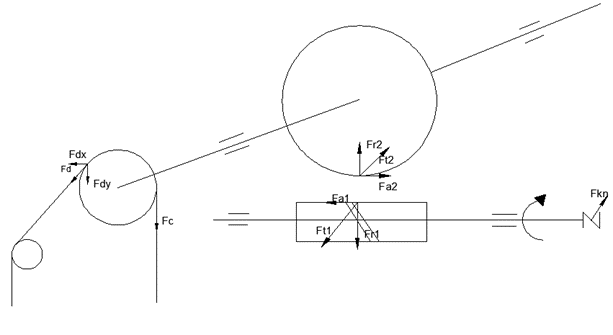
\includegraphics[width=16cm,height=9cm]{Image/force_diagram.png}}
    \caption[General force diagram]{\bfseries \fontsize{12pt}{0pt}\selectfont General force diagram}
    \label{figure1}
\end{figure}

In which:\\
- Ft1 - tangential force acting on the guide shaft I
(Ft1 is parallel to axis II, opposite rotation n1)\\
- Ft2 - tangential force acting on axis II
(Ft2 is parallel to axis I, arc of rotation n2)\\
We have the values of the forces:\\

$$F_{a1}=F_{t2}=\frac{{2\times T}_2}{d_2}=\frac{2\times593464.29}{301.5}=3936.74\left(Nmm\right)$$
$$F_{a2}=F_{t1}=\frac{2\times T_1}{d_1}=\frac{2\times7396.17}{3}=4930.78\left(Nmm\right)$$
$$F_{r1}=F_{r2}=F_{a1}\times\frac{tan\propto}{cos\gamma}=3936.74\times\frac{tan20}{cos2.08^{\circ}}=1433.67\left(Nmm\right)$$
\textbf{a.	Preliminary calculation of shaft diameter:}\\
Consider the case of full load.\\
Preliminary selection of screw diameter.
$$d_1\geq\left(0,8\ldots.1,2\right).d_{dc}=\left(0,8\ldots.1,2\right).28=\left(22,4\ldots33,6\right)mm$$
Choose d1 = 31 mm\\
Preliminary selection of worm gear diameter:
$$d_2\geq\sqrt[3]{\frac{T_2}{0,2.\left[\tau\right]}}=\sqrt[3]{\frac{1042382,5}{0,2.30}}=55,8mm,\ with τ=30 $$
Choose d2 = 60 mm\\
Look up table 10.2[I] to choose the width of the bearing:\\
			$$ b_{01} = 21 mm,  b_{02} = 31 mm	$$\\
\textbf{b.	Diagram of distance calculation for screw reducers}\\
\textbf{ Axis I} \\
Look up table 10.3[I] we have: Choose k3 = 15 mm, $h_n$ = 15 mm
$$l_{11}=d_{aM2}=304mm;l_{13}=\frac{l_{11}}{2}=\frac{304}{2}=152mm	$$
Half articulated wheel hub length :
$$l_{mkn}=l_{m12}=l_m=2.d=2.35=70mm;\;l_{12}=-l_{c12}$$
$$\bigm l_{c12}=0,5(l_{m12}+b_0)+k_3+h_n=0,5(70+21)+15+15=75,5mm$$
$$l_{12}=-l_{c12}$$
$$\bigml_{c12}=0,5(l_{m12}+b_0)+k_3+h_n=0,5(70+21)+15+15=75,5mm$$
\begin{figure}[!ht]
    \centering
     % \centerline{\includegraphics[width=1.1\textwidth, height = 1.5cm]{s_TTCD_data.png}}
   \centerline{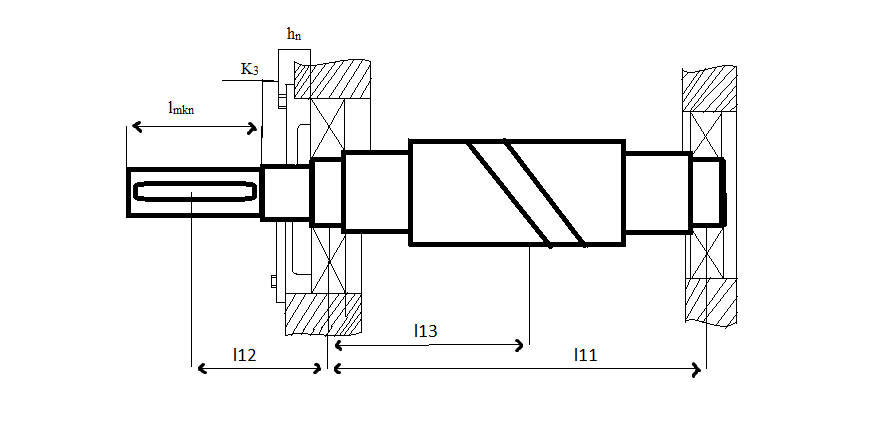
\includegraphics[width=16cm,height=9cm]{Image/axis1.png}}
    \caption[Axis II]{\bfseries \fontsize{12pt}{0pt}\selectfont Axis I}
    \label{figure1}
\end{figure}

\textbf{ Axis II} \\ 
With:
$k_1=10mm$;
$\bigmk_2=10mm$ 	
$k_3=10mm$
$\bigmh_n=15mm$
With  $	d_2 = 60 mm \rightarrow b_0=31mm$\\
\begin{figure}[!ht]
    \centering
     % \centerline{\includegraphics[width=1.1\textwidth, height = 1.5cm]{s_TTCD_data.png}}
   \centerline{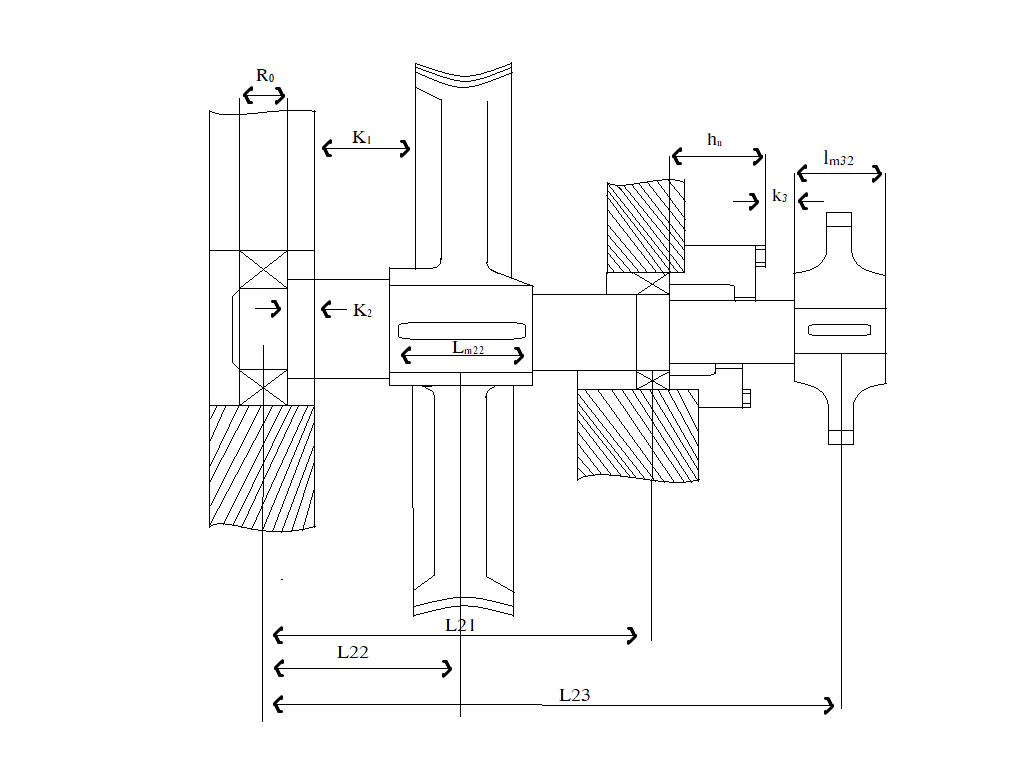
\includegraphics[width=16cm,height=9cm]{Image/axis2.png}}
    \caption[Axis II]{\bfseries \fontsize{12pt}{0pt}\selectfont Axis II}
    \label{figure1}
\end{figure}
\textbf{c. Determine the diameters and lengths of the shaft segments} 
\textbf{ Axis I}\\
Select half articulated wheel hub length $l_m = 120 mm$
\begin{figure}[!ht]
    \centering
     % \centerline{\includegraphics[width=1.1\textwidth, height = 1.5cm]{s_TTCD_data.png}}
   \centerline{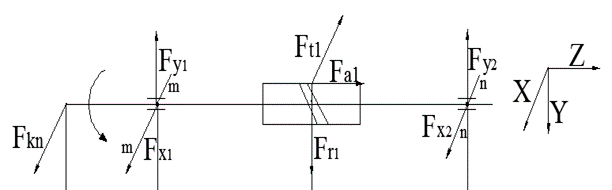
\includegraphics[width=16cm,height=5cm]{Image/Picture2.png}}
    %\caption[]{\bfseries \fontsize{12pt}{0pt}\selectfont }
    \label{figure1}
\end{figure}
We have:\\
$$M_{1x}={-F}_{r1}\times\left(I_{11}-I_{13}\right)+F_{y2}\times I_{11}-F_{a1}\times\frac{d_1}{2}=0$$
$$F_{y2}=\frac{F_{r1}\times\left(I_{11}-I_{13}\right)+F_{a1}\times\frac{d_1}{2}}{I_{11}}=\frac{2643,11\times152+7238,763\times\frac{70,4}{2}}{304}=2159,7275N$$
$$F_{y1}=F_{r1}-F_{y2}=2643,11-2159,7275=483,382N$$
$$M_{1y}=F_{t1}\times I_{13}+F_{kn}{\times I}_{12}-F_{x2}\times2\times I_{13}=0$$
$$F_{x2}=\frac{F_{t1}.\times+F_{kn}\times I_{12}}{2.I_{13}}=\frac{698,397\times152+617,626\times75}{304}=501,5733(N)$$
$$F_{x1}=F_{kn}+F_{x2}-F_{t1}=617,626 + 501,5733 -698,397=420,8023 N$$
\textbf{d.	Calculate the bending moment at the cross-sections}
$$	M_j=\sqrt{{M_{yj}}^2+{M_{xj}}^2}$$
Consider cross section m – m at 1 :\\
$$M_{mx}=F_{y2}\times I_{13}= 2159,7275\times152=328278(Nmm)$$
$$M_{my}=F_{x2}\times I_{13}=501,5733.152=76239,1416\left(Nmm\right)$$
$$M_m=\sqrt{M_{mx}^2+M_{my}^2}=\sqrt{{328278}^2+{76239,14}^2}=337014,6165\left(Nmm\right)$$
With T1 = 26189,92 (Nmm)
$$M_{td}=\sqrt{M_m^2+0,75\times T_1^2}=\sqrt{{337014,61}^2+{0,7\times.26189,92}^2}=337776,96\left(Nmm\right)$$
Consider the section n – n at 2:
$$M_{nx}=0;M_{ny}=F_{kn}.I_{12}=617,62.75=46321,5\ (Nmm)$$
$$\rightarrow M_n=M_{ny}=46321,5 (Nmm)$$
\textbf{e.	 Calculate shaft diameter at 2 sections}\\
At the cross section m - m: taken by the diameter of the screw thread foot :\\
$d_{m-m} = 70,4 mm$\\
At the cross section n - n :
$$d=\sqrt[3]{\frac{M_{td}}{0,1\left[\sigma\right]}}=\sqrt[3]{\frac{337776,96}{0,1.55}}=39,45$$
With $[\sigma]=55$ check table 10.5 shaft material made of 45 tempered steel.\\
 Choose $\Rightarrow d = 24 mm$\\
	 Choose the diameter of the fitting place to be d = 31 mm\\
	The diameter at the n – n section is taken no more than 5 mm larger than the diameter of the fitting, so choose d= 36 mm.\\
\subsection{Calculation of bearing selection for shaft I}
Select bearing type, calculate Fr at the supports 1 and 2
$$F_{r1}=\sqrt{{F^2}_{x1}+{F^2}_{y1}}=\sqrt{{420,80}^2+{483,38}^2}=640,884N$$
$$F_{r2}=\sqrt{{F^2}_{x2}+{F^2}_{y2}}=\sqrt{{501,57}^2+{2159,72}^2}=2217,19N$$
$$F_{at}=7238,77N$$
Consider $ \frac{F_{at}}{F_{r2}}=\frac{7238,77}{2217,19}=3,26$\\
For screw shafts, it is mandatory to use tapered roller bearings and at the same time, the screw shaft must arrange bearings as follows:\\%chen hinh vao
\textbf{Including:}\\
A bearing "1" so that the screw can move axially to avoid curvature of the screw due to thermal expansion.\\
A pair of "2" double tapered roller bearings that fix the shaft.\\
	Select bearing precision grade : accuracy grade 0\\
\subsubsection{Select the bearing type: single row ball bearing }
Look up table P2.7 T.254[I] We have the symbol of a light-weight single row ball bearing :208\\
We have :\\
Inner diameter d = 40 mm\\
Outer diameter D = 80 mm\\
Dynamic load capacity C = 25.6 kN\\
Calculation load capacity C0 = 18.1 kN\\
Experimental coefficient: $1.5\times \tan \alpha=1.5\times \tan10.83= 0.29$  \\
Test the load capacity of the drive\\
We have : $Q=(X.V.F_{r1}+YF_a).k_t.k_d$
In which, for ball bearings bearing radial force X = 1\\
Bearing bearing does not bear axial force, so Y = 0\\
The inner ring of the bearing rotates so V = 1\\
Factor taking into account the effect of temperature kt = 1 (because t$\le100^0c)$\\
light impact load characteristics kd = 1
$$\rightarrow Q=F_{r1}\times k_d\times k_t=640,884\times1\times1=640,89\ N$$
$$L=\frac{60\times n\times L_h}{{10}^6}=\frac{60\times1425\times12000}{{10}^6}=1026 \;( million\; revolutions) $$
Where: n is the number of shaft revolutions (rpm)\\
$Lh$ is the lifespan (hours)\\
Dynamic load capacity required with rolling bearing:\\
$$C_d^{yc}=Q\times L^\frac{1}{3}=640,884\times{1026}^\frac{1}{3}=6463,9\ N\ \approx4,46\ kN\ $$
$\Rightarrow{C_d}^{yc}<C=37,8kN $ (satisfied)
\subsubsection{Calculation of choosing a tapered roller bearing}
	 Choose a wide-range single-row tapered roller bearing with:\\
		Symbol: 7609\\
		Dynamic load capacity: C = 104 kN\\
        Static load capacity: C0 = 90.5 kN\\
        $\alpha=11^0 $\\
    Draw a bearing diagram ( using O bearings).
\begin{figure}[!ht]
    \centering
     % \centerline{\includegraphics[width=1.1\textwidth, height = 1.5cm]{s_TTCD_data.png}}
   \centerline{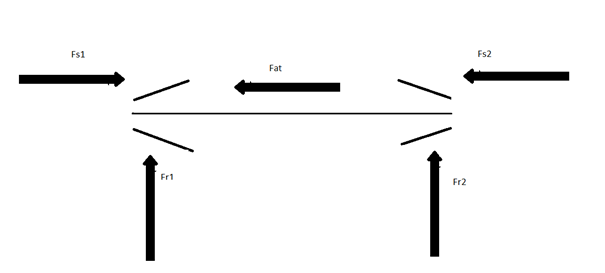
\includegraphics[width=16cm,height=7cm]{Image/Picture3.png}}
    %\caption[]{\bfseries \fontsize{12pt}{0pt}\selectfont }
    \label{figure1}
\end{figure}
Calculate e:\\
$$e=1.5\times \tan \alpha=1.5\times \tan10.83= 0.29$$
According to (11.7) axial force due to radial force on rolling bearings:\\
$$F_{s1}=F_{s2}=0,5\times0,83\times e\times F_{r2}=0,5\times0,83\times0,29\times2217,19
=266,84\ (N) $$
( For screw Fr =0,5 Fr2)\\
Calculate $ \sum F_{a1};\sum F_{a2}$
$$\sum{F_{a1}=\left|F_{s2}+F_{at}\right|=\left|266,84+7238,77\right|=7505,61\ (N)}$$
$$\sum{F_{a2}=\left|F_{s2}-F_{at}\right|=\left|266,84-7238,77\right|=-6971,93\ (N)}$$
Calculate $ F_{a1};F_{a2}$\\
$$F_{a1}=Max(F_{s1};\sum{F_{a1})=7505,61}$$
$$F_{a2}=Max(F_{s2};\sum{F_{a2})=6971,93}$$
Calculate Q1; Q2 (conventional dynamic load)\\
	Consider $ \ \frac{F_{a1}}{0,5\times V\times F_{r2}}=\frac{7505,61}{0,5\times2217,19}=6,77$ > e, so:\\
	X1 = 0,4; Y1 = 0,4.cotg110 = 2,06
$$	\Rightarrow Q_1=(X.V.F_{r1}+YF_{a1}).k_t.k_d$$
$$ =\left(0,4\times0,5\times2217,19+2,06\times7505,61\right)\times1\times1$$
$$=15904,99\ (N)$$
Dynamic load testing:\\
Q = Max(Q1,Q2) = Q1 = 15904,99 N\\
$$L=\frac{60\times n\times L_h}{{10}^6}=\frac{60\times1425\times12000}{{10}^6}=1026 \; ( million\; revolutions)$$
Dynamic load capacity required for rolling bearing:\\
$$C_d^{yc}=Q\times L^\frac{3}{10}=15904,99\times{1026}^\frac{3}{10}=127314,43\ N\ \approx127,31\ kN\ $$
${C_d}^{yc}>C $ unsatisfactory\\
We reduce the bearing life: every $\frac{L_h}{3}$ then change the bearing 1 time.\\
 Therefore : $L = \frac{1026}{3}=342$
 $${\rightarrow C}_d^{yc}=Q\times L^\frac{3}{10}=15904,99\times{342}^\frac{3}{10}=91567,47\ N\ \approx91,56\ kN\ $$
$ {C_d}^{yc}<C=104(kN) $ satisfied
\subsection{Preliminary calculation of shaft diameter II and roller bearing II}
\subsubsection{Determine the preliminary diameter}
$$d_{2sb}=3TII0,2[τ] pick [\tau]=22÷28>[τ] axis I \Rightarrow[\tau]=25$$
$\Rightarrow d_{2sb}=\sqrt[3]{\frac{1043282,5}{0,2.25}}=59,3 (mm) $ => choose $d_{2sb}$  = 60 mm\\
Choose $d3 <d2sb \Rightarrow $ choose d3  = 55 mm\\
d0 = d2sb = 60 mm\\
d1 > d0 choose d1 = 65 mm\\
Draw the shaft texture:\\
\begin{figure}[!ht]
    \centering
     % \centerline{\includegraphics[width=1.1\textwidth, height = 1.5cm]{s_TTCD_data.png}}
   \centerline{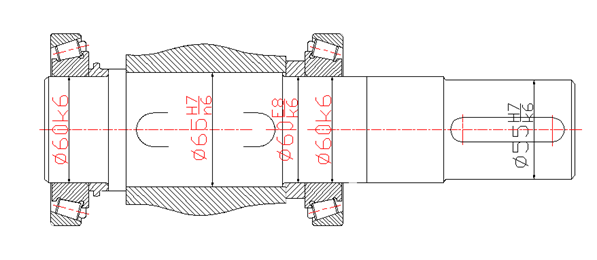
\includegraphics[width=16cm,height=7cm]{Image/Picture4.png}}
    %\caption[]{\bfseries \fontsize{12pt}{0pt}\selectfont }
    \label{figure1}
\end{figure}
\subsubsection{Select the bearing at the 0 and 2 buttons}
Choose a light-sized 7612 tapered roller bearing with d = d0 = 60 mm\\
Tapered roller bearing has D = 130 mm; B = 46 mm\\
\section{Structural calculation of the speed reduction box}
\subsection{Worm gear texture}
From the picture 14-14t.16[II] and the formulas we have:\\
	Shaft distance a = 190 mm ,\\
	Width of worm gear b2 = 60 mm ,\\
	Sewing length lm  = 90 mm\\
	Tilt angle $\gamma$ = 5,710\\
	Diameter of top ring d a2  = 292,92 mm \\
	Diameter of dividing ring d2  = 285 mm \\
	Diameter of bottom ring df2 = 279,72 mm \\
\subsection{Screw structure }
\subsection{Gearbox structure }
- The standard of the reducer housing is high rigidity and small weight. \\
- Choosing the material for casting the reducer is gray cast iron with the symbol GX 15-32. \\
- Choose a mounting surface that passes through the center of the shaft and the body for easy mounting.  \\
Basic sizes\\
 
\newpage
%\pagenumbering{arabic} % Đánh số thứ tự 1,2,3...
\section*{CHAPTER 3\\ \vspace{0.5cm} DETAILED DESIGN AND ASSEMBLY}
\addcontentsline{toc}{section}{\numberline{}CHAPTER 3\\ \vspace{0.5cm} DETAILED DESIGN AND ASSEMBLY}

\newpage
%\pagenumbering{arabic} % Đánh số thứ tự 1,2,3...
\section*{CHAPTER 4\\ \vspace{0.5cm} SIMULATION}
\addcontentsline{toc}{section}{\numberline{}CHAPTER 4\\ \vspace{0.5cm} SIMULATION}

\newpage
\section*{Reference}
1.	Chi tiết máy ,tập I và II :           \\       
Nguyễn Trọng Hiệp\\
          			   	   Nhà xuất bản giáo dục - 2001\\
1.	Tính toán thiết kế hệ dẫn động cơ khí  tập I va II\\
PGS . TS .Trịnh Chất – TS . Lê Văn Uyển\\
               		 Nhà xuất bản giáo dục - 2000\\
2.	Hướng dẫn làm bài tập dung sai \\
 PGS . TS . Ninh Đức Tốn – TS . Đỗ Trọng Hùng \\
             		  Trường ĐHBK Hà Nội – 2000.\\

\end{titlepage}
\end{document}
